\chapter{Recognition on SpiNNaker}
\label{cha:rsp}

\section{Moving from Perceptrons to Spiking Neurons}
It remains a challenge to transform traditional artificial neural networks into spiking ones.
There are attempts~\cite{la2008response}~\cite{burkitt2006review} to estimate the output firing rate of the LIF neurons (Equation~\ref{equ:lif}) under certain conditions. 
%For the model illustrated above, there are two types of synaptic connection: one-to-one connections in the retina layer and N-to-one connections in all the convolutional layers (the pooling layer is also included). 
%For the retina layer, 1) the problem is: what is the connection weight between two single LIF neurons to make a post-synaptic neuron fire whenever the pre-synaptic neuron generates a spike? 
%While for the convolutional neurons, 2) given the input spike rates, LIF neuron parameters and the output spiking rate, what are the corresponding weights between the two layers?
\begin{equation}
\frac{\D \: V(t)}{\D\:  t}=-\frac{V(t)-V_\mathit{rest}}{\tau_m}+\frac{I(t)}{C_m}
\label{equ:lif}
\end{equation}
The membrane potential $V$ changes in response to input current $I$, starting at the resting membrane potential  $V_{rest}$, where the membrane time constant is $\tau_m = R_mC_m$, $R_m$ is the membrane resistance and $C_m$ is the membrane capacitance.

Given a constant current injection $I$, the response function, i.e. firing rate, of the LIF neuron is
\begin{equation}
\lambda_\mathit{out}=
\left [ t_\mathit{ref}-\tau_m\ln \left ( 1-\frac{V_{th}-V_\mathit{rest}}{IR_m}  \right )\right ]^{-1}
\label{equ:consI}
\end{equation}
when $IR_m>V_{th}-V_{rest}$, otherwise the membrane potential cannot reach the threshold $V_{th}$ and the output firing rate is zero. 
The absolute refractory period $t_\mathit{ref}$ is included, where all input during this period is invalid.
In a more realistic scenario, the post-synaptic potentials (PSPs) are triggered by the spikes generated from the neuron's pre-synaptic neurons other than a constant current.
Assume that the synaptic inputs are Poisson spike trains, the membrane potential of the LIF neuron is considered as a diffusion process. Equation~\ref{equ:lif} can be modelled as a stochastic differential equation referring to Ornstein-Uhlenbeck process,
\begin{equation}
\tau_m\frac{\D\:V(t)}{\D\:  t}=-\left[V(t)-V_\mathit{rest}\right] + \mu + \sigma\sqrt{2\tau_m}\xi (t)
\label{equ:sde}
\end{equation}
where
\begin{equation}
\begin{array}{l}
\mu=\tau_m(\mathbf{w_E\cdot\lambda_E}-\mathbf{w_I\cdot\lambda_I})
\\
\\
\sigma ^{2} = \frac{\tau_m}{2}\left(\mathbf{w_E^{2}\cdot\lambda_E}+\mathbf{w_I^{2}\cdot\lambda_I}\right)
\end{array}
\label{equ:ou}
\end{equation}
are the conditional mean and variance of the membrane potential.
The delta-correlated process $\xi(t)$ is Gaussian white noise with zero mean, $\mathbf{w_E}$ and $\mathbf{w_I}$ stand for the weight vectors of the excitatory and the inhibitory synapses, and $\mathbf{\lambda}$ represents the vector of the input firing rate.
The response function of the LIF neuron with Poisson input spike trains is given by the Siegert function~\cite{siegert1951first}, 
\begin{equation}
\lambda_\mathit{out}=\left(\tau_\mathit{ref} + \frac{\tau_Q}{\sigma_Q}\sqrt{\frac{\pi}{2}} \int_{V_\mathit{rest}}^{V_\mathit{th}}du \:\exp \left(\frac{u-\mu_Q}{\sqrt2\sigma_Q} \right )^{2}\left[1+erf \left(\frac{u-\mu_Q}{\sqrt2\sigma_Q} \right ) \right ]\right)^{-1}
%\begin{split}
%\lambda_\mathit{out}=\left(\tau_\mathit{ref} + \frac{\tau_Q}{\sigma_Q}\sqrt{\frac{\pi}{2}} \int_{V_\mathit{rest}}^{V_\mathit{th}}\D u \:\exp \left(\frac{u-\mu_Q}{\sqrt2\sigma_Q} \right )^{2}\left[1+\mathrm{erf} \left(\frac{u-\mu_Q}{\sqrt2\sigma_Q} \right ) \right ]\right)^{-1}
%\end{split}
%\label{equ:sgt}
\end{equation}
%\begin{align}
%\lambda_\mathit{out} &=\left(\tau_\mathit{ref} + \frac{\tau_Q}{\sigma_Q}\sqrt{\frac{\pi}{2}} \int_{V_\mathit{rest}}^{V_\mathit{th}}\D\,u \:\exp \left(\frac{u-\mu_Q}{\sqrt2\sigma_Q} \right )^{2} \right. \nonumber \\
%&\qquad \left. \vphantom{\int_t} \cdot  \left[1+\mathrm{erf} \left(\frac{u-\mu_Q}{\sqrt2\sigma_Q} \right ) \right ]\right)^{-1}
%\label{equ:sgt}
%\end{align}
where $\tau_Q, \mu_Q, \sigma_Q$ are identical to $\tau_m, \mu, \sigma$ in Equation~\ref{equ:ou}, and erf is the error function.

Still there are some limitations on the response function. 
For the diffusion process, only small amplitude (weight) of the PostSynaptic Potentials (PSPs) generated by a large amount of input spikes (high spiking rate) work under this circumstance; 
plus, the delta function is required, i.e. the synaptic time constant is considered to be zero. Thus only a rough approximation of the output spike rate has been determined.
Secondly, given different input spike rate to each pre-synaptic neurons, the parameters of the LIF neuron and the output spiking rate, how to tune every single corresponding synaptic weight remains a difficult task.


\section{Live Recognition}
\begin{figure}[h!]
	\centering
	\begin{subfigure}[t]{0.48\textwidth}
		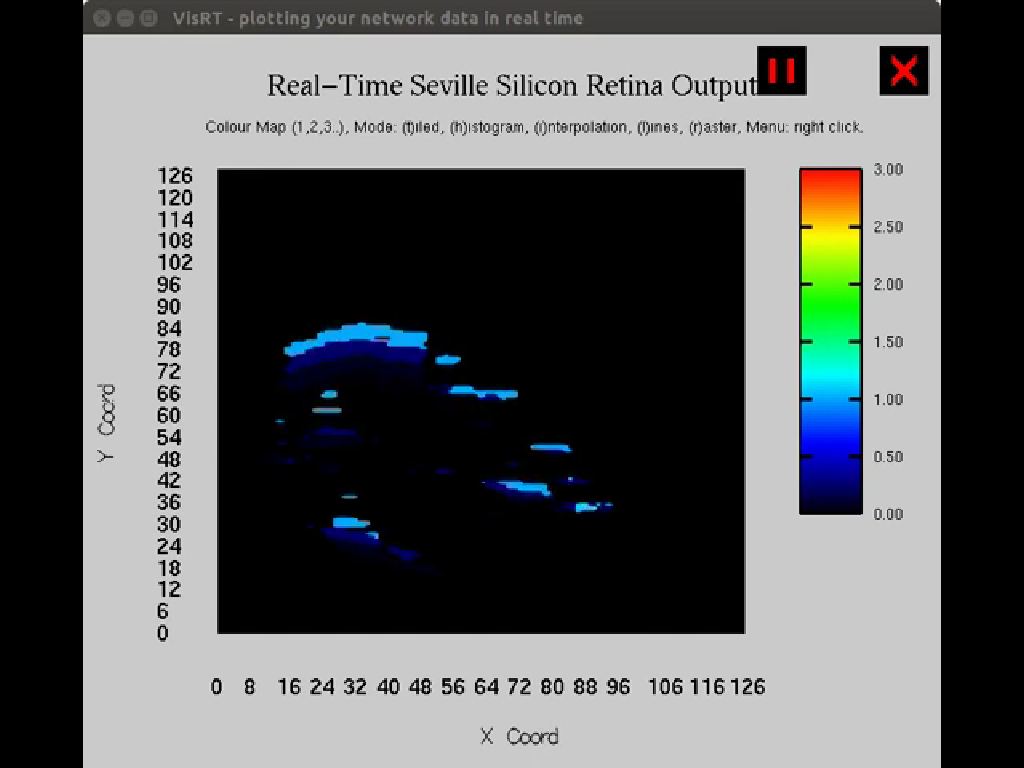
\includegraphics[width=\textwidth]{pics/live1_colour.png}
		\caption{Neural responses of the Gabor filter layer orienting to the horizontal direction~\cite{video1} }
		\label{fig:live1}
	\end{subfigure}
	\begin{subfigure}[t]{0.48\textwidth}
		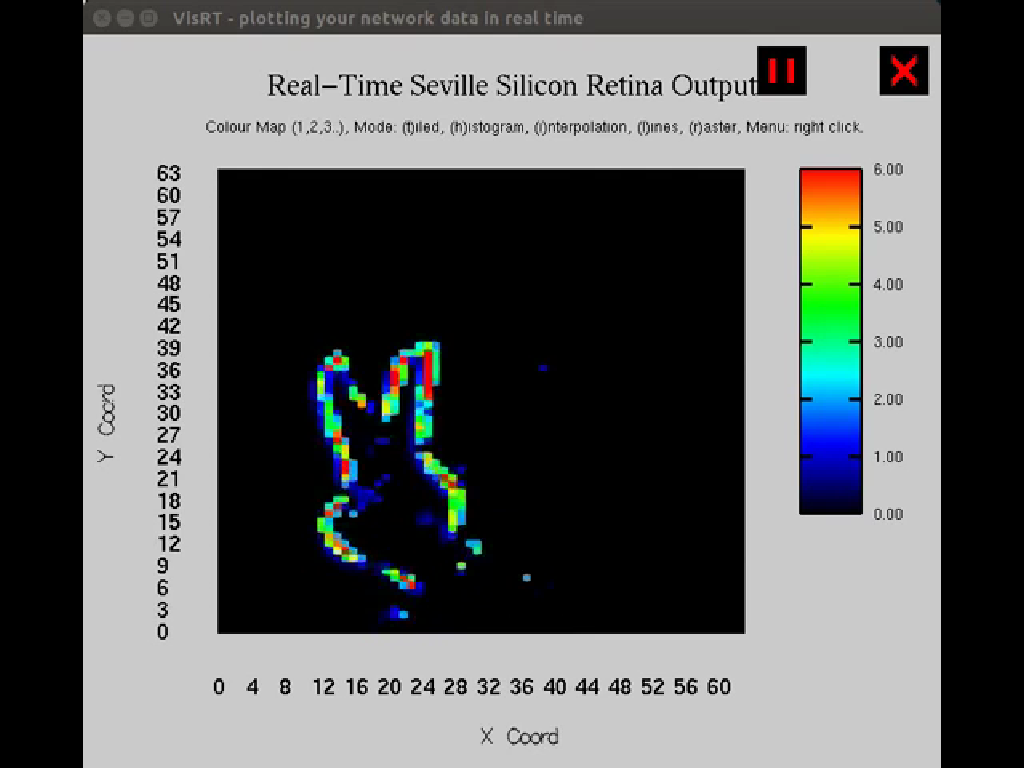
\includegraphics[width=\textwidth]{pics/live2_colour.png}
		\caption{Neural responses of the integrate layer~\cite{video2}}
		\label{fig:live2}
	\end{subfigure}
	\\
	\begin{subfigure}[t]{\textwidth}
		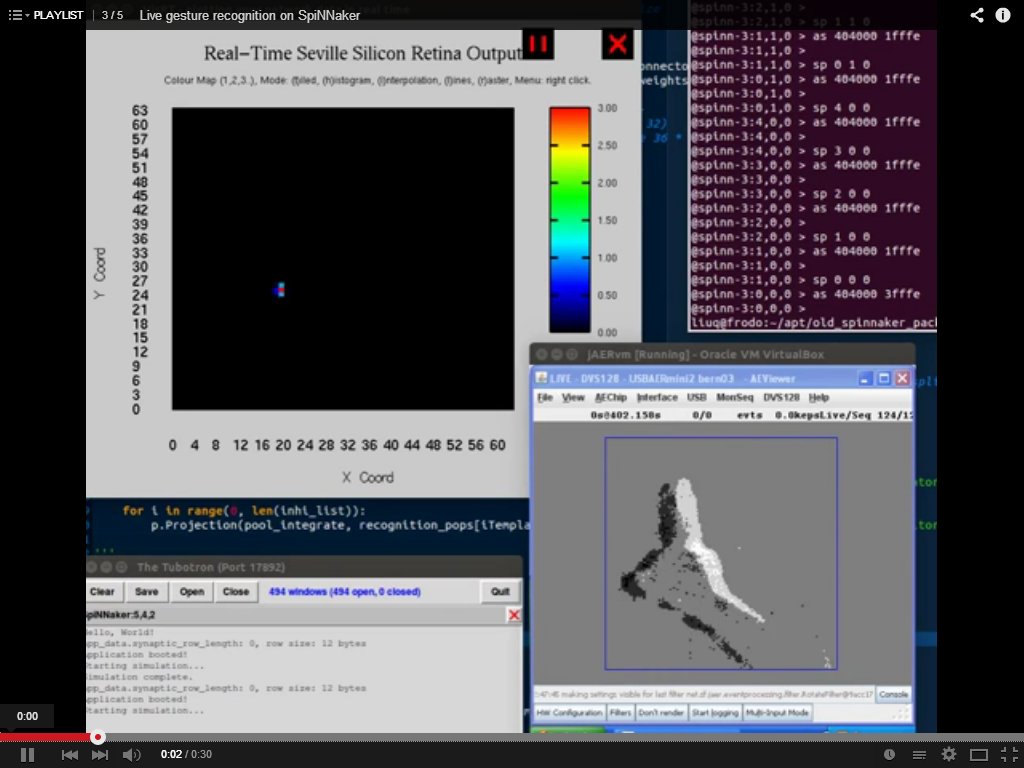
\includegraphics[width=\textwidth]{pics/live_colour.png}
		\caption{Snapshot of the neuron responses of the template matching layer~\cite{video3}}
		\label{fig:live3}
	\end{subfigure}	
	
	\caption{Snapshots of the real-time dynamic posture recognition system on SpiNNaker.
	}
	\label{fig:live}
\end{figure}
We implemented the prototype of the dynamic posture recognition system on SpiNNaker using LIF neurons. 
The input retina layer consists of 128$\times$128 neurons; 
each Gabor filter has 112$\times$112 valid neurons, since the kernel size is 17$\times$17; 
each pooling layer is as big as 36$\times$36, convolving with five template kernels (21$\times$21); 
thus, the recognition populations are 16$\times$16 neurons each. Altogether $74,320$ neurons and $15,216,512$ synapses, use up to 19 chips (290 cores) on a 48-node board, see Table~\ref{tbl:m1}. Regarding the lower resolution of 32$\times$32 retinal input, the network (Table~\ref{tbl:m2}) consists of $5,925$ neurons and $318,420$ synapses taking up only two chips (31 cores) of the board.

Figure~\ref{fig:live} shows snapshots of neural responses of some populations during real-time recognition.
Figure~\ref{fig:live1} is a snapshot of the Gabor population which prefers the horizontal direction, given the input posture of a `Fist'; and Figure~\ref{fig:live2} shows the activity of the neurons in the integration layer, given a 'Victory Sign'.
And the active neurons in the visualiser in Figure~\ref{fig:live3} are pointing out the position of the recognised pattern the `Index finger'. 
All the supporting demonstrative videos can be found on YouTube~\cite{video1, video2, video3}. %\footnote{\url{
%https://www.youtube.com/watch?v=PvJy6RKAJhw&feature=youtu.be&list=PLxZ1W-Upr3eoQuLxq87qpUL-CwSphtEBJ, http://youtu.be/FZJshPCJ1pg?list=PLxZ1W-Upr3eoQuLxq87qpUL-CwSphtEBJ, http://youtu.be/yxN90aGGKvg?list=PLxZ1W-Upr3eoQuLxq87qpUL-CwSphtEBJ}}.


\section{Recognition of Recorded Data}
To compare with the results of the experiments carried out with Matlab (in Section~\ref{sec:exp}), the same recorded retinal data is conducted into SpiNNaker.
Only Model 1 is tested on the neuromorphic hardware platform, since tracking is still need to investigate using SNN (for Model 2) in the future. 
The recorded data is presented as spike source array in the system with 128$\times$128 input (see Figure~\ref{fig:ssa}) while the data is forwarded to a sub-sampling layer of 32$\times$32 resolution in the system of the smaller network (see Figure~\ref{fig:ssa32}). 
The output spikes generated from the recognition populations with time are shown in Figures~\ref{fig:rps} and \ref{fig:rps32} for full resolution and lower systems respectively. 
More spikes are generated during the period when the preferred input posture is shown. 


\begin{figure}[h!]
\centering
	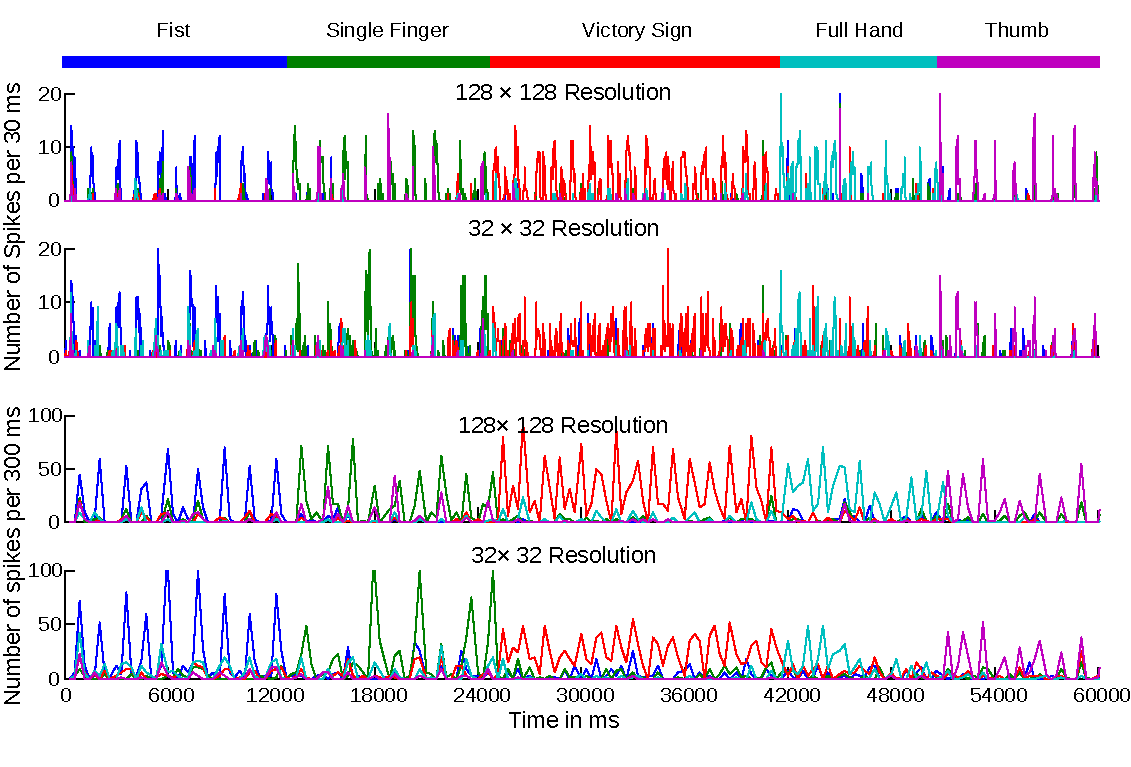
\includegraphics[width=\textwidth]{pics/rateSpiNN.pdf}
	\caption{Real-time neural responses of two experiments on SpiNNaker with time to the same recorded postures.
	These two experiments only differ in input resolution.
	The result of the high input resolution test is plotted the first with a sample frame of 30~ms; 
	while the 3rd plot shows the same result with a sample frame of 300~ms.
	The other two plots refer to the smaller input resolution.
	Every point represents the over all number of spikes of a specific population (different colour) in a `frame'.
	}
	\label{fig:spikerec}
\end{figure}

Correspondingly, the spiking rates of each recognition population is sampled into frames (Figure~\ref{fig:spikerec}) to make a comparison with the Matlab simulation. 
Each colour represents one recognition population, and the spike activity goes higher when the input posture matches the template. 
Firstly, the spike rates are sampled into 30~ms frames which is in accordance with the Matlab experiments.
In the Matlab simulation, the templates are trained with cut frames and so the test images are also fixed to the same length frames.
Otherwise, the recogniser will not work properly because of the replications of the moving posture.
Contrasting this, the spiking rates can be sampled to various frame lengths.
Thus, the other two plots in the figure illustrate the classification in a wider window of 300~ms.
From Table~\ref{tbl:srr}, the recognition and rejection rates are quantified as percentages.

\begin{table}[h!]
	\centering
	\caption{Real-time recognition results on SpiNNaker in \%}
	\begin{tabular}{p{0.15\textwidth}|p{0.1\textwidth}<{\centering}|p{0.11\textwidth}<{\centering}|p{0.11\textwidth}<{\centering}|p{0.11\textwidth}<{\centering}|p{0.11\textwidth}<{\centering}}
		%Line 1
		\Xhline{1.2pt}
		\multicolumn{2}{c|}{}	& \multicolumn{2}{c|}{\textbf{30~ms per frame}}  
		& \multicolumn{2}{c}{\textbf{300~ms per frame}}
		\\ \cline{3-6}
		%Line 2
		\multicolumn{2}{c|}{}	& \tabincell{c}{High \\ Resolution}
		& \tabincell{c}{Low \\ Resolution}
		& \tabincell{c}{High \\ Resolution}
		& \tabincell{c}{Low \\ Resolution}
		\\ \Xhline{1.2pt}
		%Line 3-4	
		\multirow{2}{*}{\tabincell{l}{\textbf{Fist}}}
		& Correct & 91.78	& 78.02	& 100	& 92.31
		\\ \cline{2-6}
		& Reject  & 82.78 & 78.54 	& 70.73	& 68.29
		\\ \hline
		%Line 5-6
		\multirow{2}{*}{\tabincell{l}{\textbf{Index Finger}}}
		& Correct & 78.25	& 78.25	& 88.24	& 72.22
		\\ \cline{2-6}
		& Reject & 80.46	& 73.56 	& 57.50	& 55.00
		\\ \hline
		%Line 7-8
		\multirow{2}{*}{\tabincell{l}{\textbf{Victory Sign} }}
		& Correct & 96.48	& 86.27	& 95.00	& 92.50
		\\ \cline{2-6}
		& Reject & 64.46	& 72.68 	& 28.57	& 28.57
		\\ \hline
		%Line 9-10
		\multirow{2}{*}{\tabincell{l}{\textbf{Full Hand}}}
		& Correct & 85.29	& 60.78	& 90.00	& 75.00
		\\ \cline{2-6}
		& Reject & 67.31	& 83.65 	& 35.48	& 61.29
		\\ \hline
		%Line 10-11
		\multirow{2}{*}{\tabincell{l}{\textbf{Thumb up}}}
		& Correct & 84.09	& 88.10	& 91.67	& 100
		\\ \cline{2-6}
		& Reject & 87.54	& 73.81 	& 66.67	& 66.67
		\\ \hline\hline
		\multirow{2}{*}{\tabincell{l}{\textbf{Average}}}
		& Correct & 87.18	& 78.28	& 92.98	& 86.41
		\\ \cline{2-6}
		& Reject & 76.51	& 76.45 	& 51.79	& 55.96
		\\ \hline
	\end{tabular}
	\label{tbl:srr}
\end{table}

Comparing with the results of Matlab simulation (Table~\ref{tbl:rsl}), the recognition rate is about 7.6\% lower at both high and low resolutions, and the rejection rate remains the same slightly above 75\%. 
However, by changing the frame length to 300~ms recognition rates reach (93.0\% for the larger network) or exceed (86.4\% for smaller network ) the Matlab simulation, meanwhile the rejection rates also drop dramatically by 26.0\% and 22.4\%.
This is in accordance with natural visual responses, which means, the longer an object shows, the more accurate the recognition will be.
Between the two network scales there is also a smaller gap in recognition rates as the window length grows, i.e. 8.9\% and 6.6\% respectively.
%Considering the cost and performance trade-off, with only 1/10th resources required, the small network, is acceptable and can be even improved after applying tracking and learning.
%Regarding the latency between the retinal input and the recognition, we compared the spiking peak of the Matlab simulation and the real-time SpiNNaker test.
%The overall latency is about 1150~ms from a posture being shown to its recognition. 

\begin{figure}
\centering
	\begin{subfigure}[t]{0.4\textwidth}
		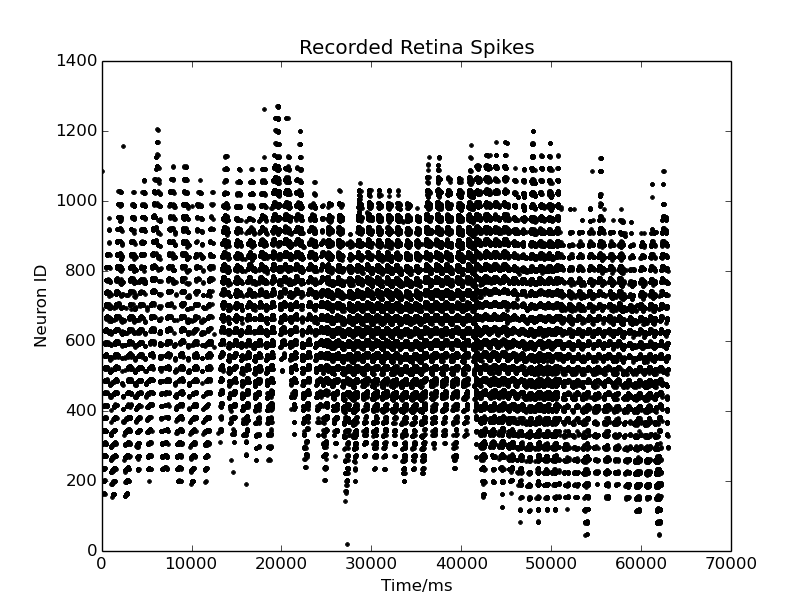
\includegraphics[width=\textwidth]{pics/figure_r.png}
	    \caption{Retinal input population }
	    \label{fig:ssa}
	\end{subfigure}
	\begin{subfigure}[t]{0.4\textwidth}
		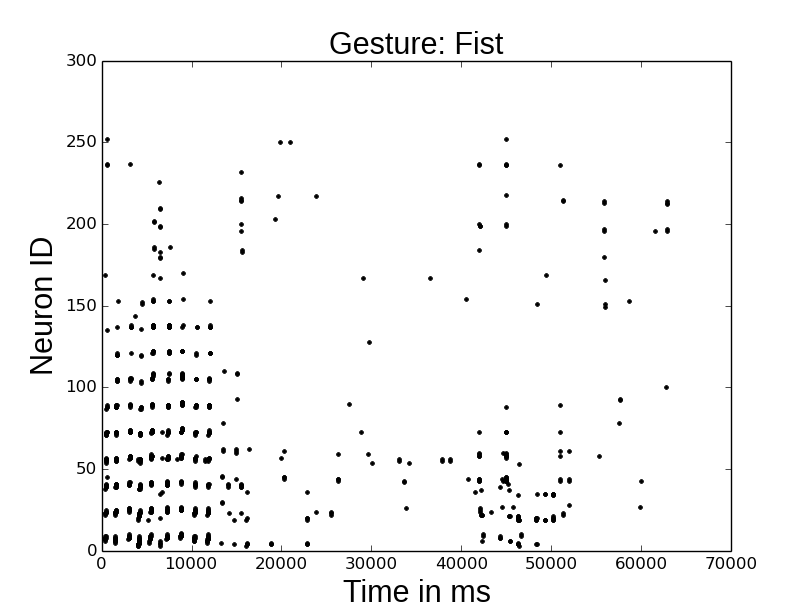
\includegraphics[width=\textwidth]{pics/figure_1.png}
		\caption{Template matching population, `Fist'}
	    \label{fig:rec0}
	\end{subfigure}
	\\
	\begin{subfigure}[t]{0.4\textwidth}
		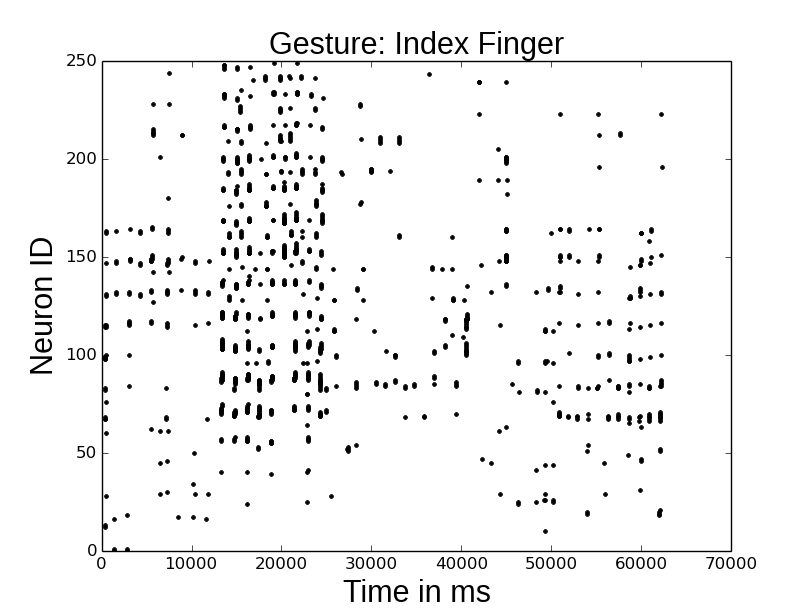
\includegraphics[width=\textwidth]{pics/figure_2.png}
		\caption{Template matching population, `Index Finger'}
	    \label{fig:rec1}
	\end{subfigure}	
	\begin{subfigure}[t]{0.4\textwidth}
		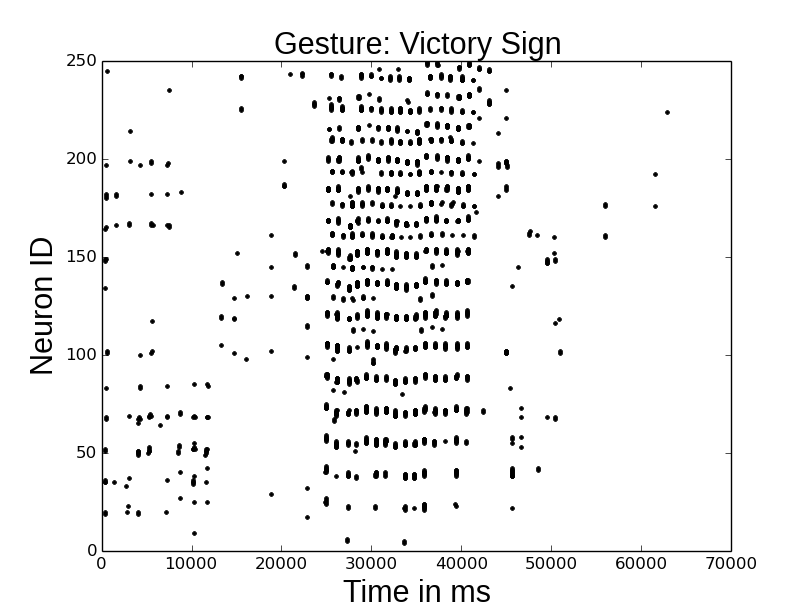
\includegraphics[width=\textwidth]{pics/figure_3.png}
		\caption{Template matching population, `Victory Sign'}
	\end{subfigure}	
	\\
	\begin{subfigure}[t]{0.4\textwidth}
		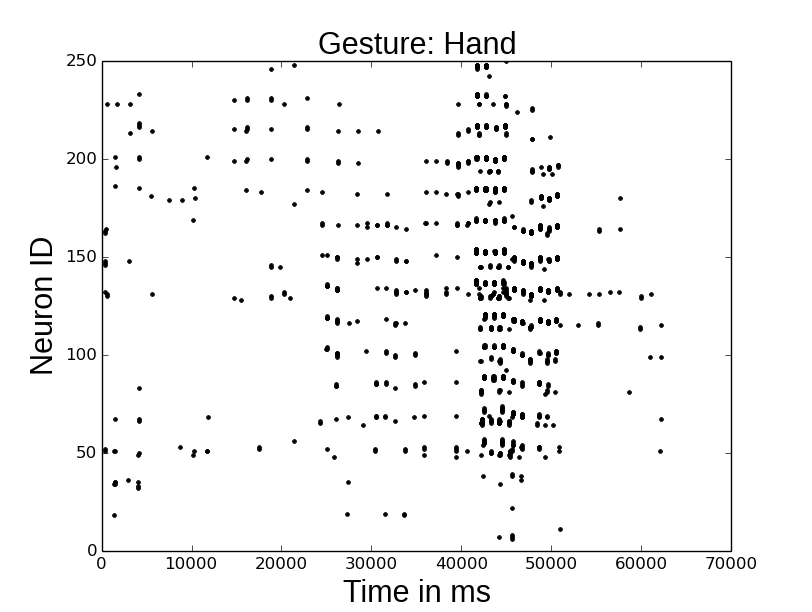
\includegraphics[width=\textwidth]{pics/figure_4.png}
		\caption{Template matching population, `Full Hand'}
	    \label{fig:rec5}
	\end{subfigure}	
	\begin{subfigure}[t]{0.4\textwidth}
		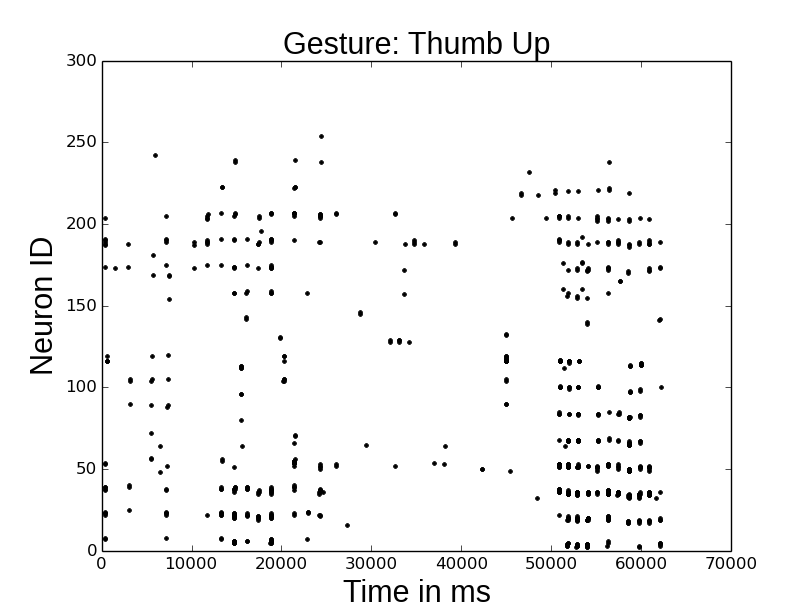
\includegraphics[width=\textwidth]{pics/figure_5.png}
		\caption{Template matching population, `Thumb Up'}
	    \label{fig:rect}
	\end{subfigure}	
\caption{Spikes captured during the live recognition of the recorded retinal input with the resolution of 128$\times$128. }
\label{fig:rps}
\end{figure}
\begin{figure}
\centering
	\begin{subfigure}[t]{0.4\textwidth}
		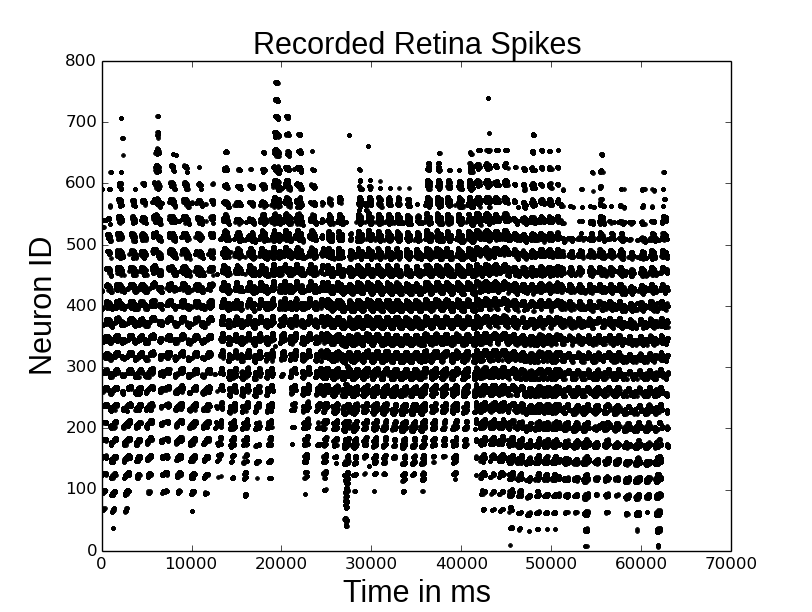
\includegraphics[width=\textwidth]{pics/figure_32_r.png}
	    \caption{Retinal input population }
	    \label{fig:ssa32}
	\end{subfigure}
	\begin{subfigure}[t]{0.4\textwidth}
		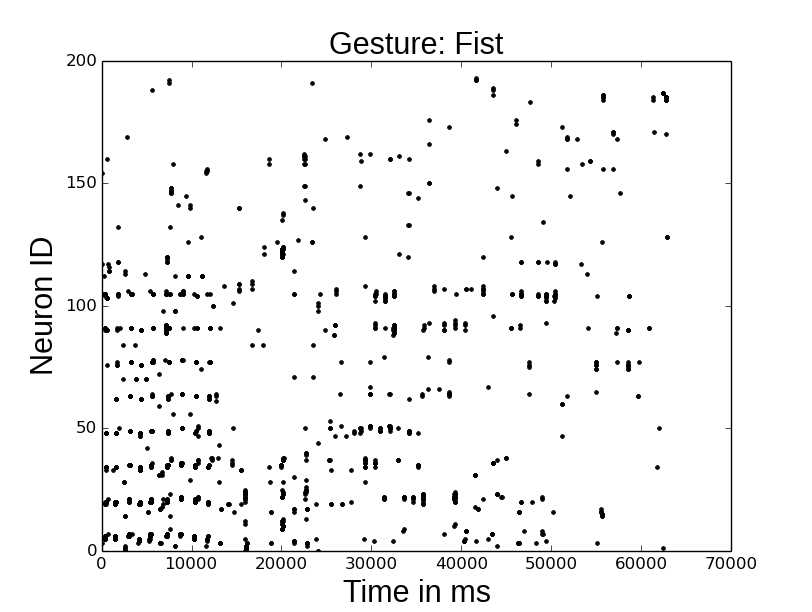
\includegraphics[width=\textwidth]{pics/figure_32_1.png}
		\caption{Template matching population, `Fist'}
	    \label{fig:rec032}
	\end{subfigure}
	\\
	\begin{subfigure}[t]{0.4\textwidth}
		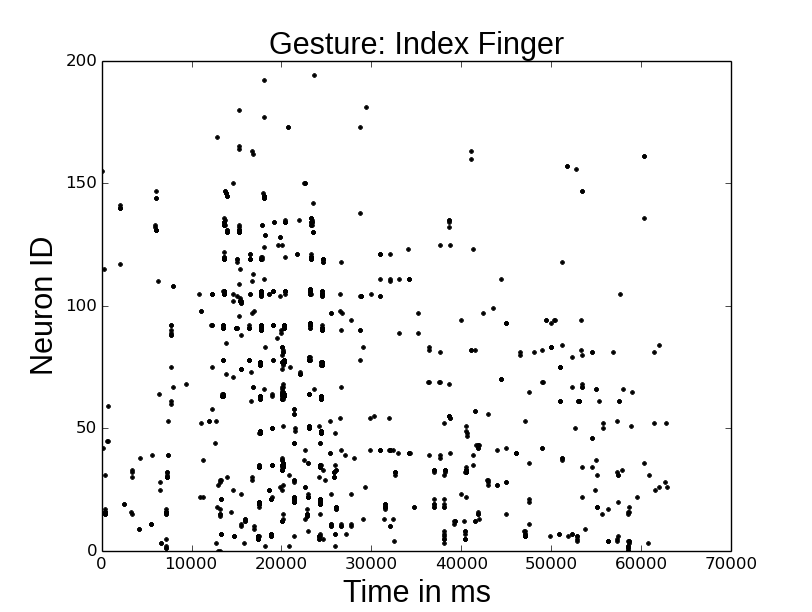
\includegraphics[width=\textwidth]{pics/figure_32_2.png}
		\caption{Template matching population, `Index Finger'}
	    \label{fig:rec132}
	\end{subfigure}	
	\begin{subfigure}[t]{0.4\textwidth}
		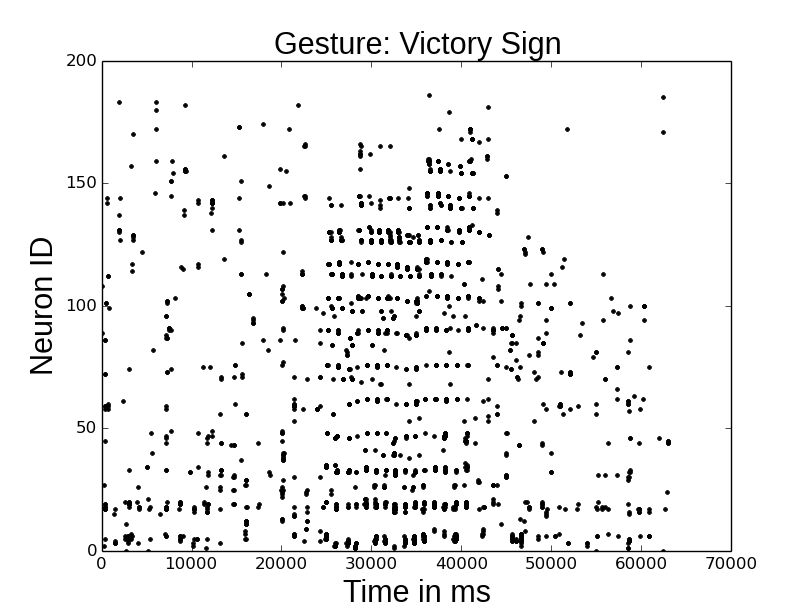
\includegraphics[width=\textwidth]{pics/figure_32_3.png}
		\caption{Template matching population, `Victory Sign'}
	\end{subfigure}	
	\\
	\begin{subfigure}[t]{0.4\textwidth}
		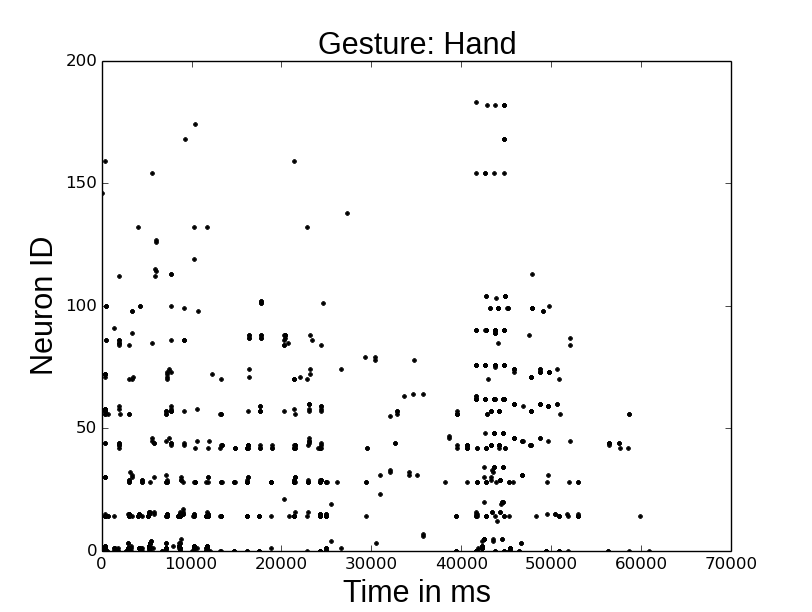
\includegraphics[width=\textwidth]{pics/figure_32_4.png}
		\caption{Template matching population, `Full Hand'}
	    \label{fig:rec532}
	\end{subfigure}	
	\begin{subfigure}[t]{0.4\textwidth}
		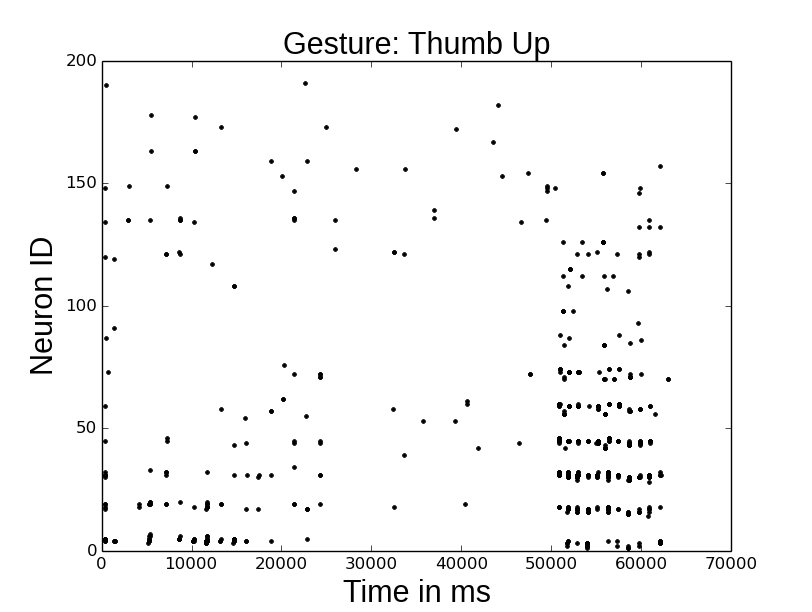
\includegraphics[width=\textwidth]{pics/figure_32_5.png}
		\caption{Template matching population, `Thumb Up'}
	    \label{fig:rect32}
	\end{subfigure}	
\caption{Spikes captured during the live recognition of the recorded retinal input with the resolution of 32$\times$32. }
\label{fig:rps32}
\end{figure}
